\section{Orthrus: Distributed Query Processing Framework}


\begin{figure}
\centering 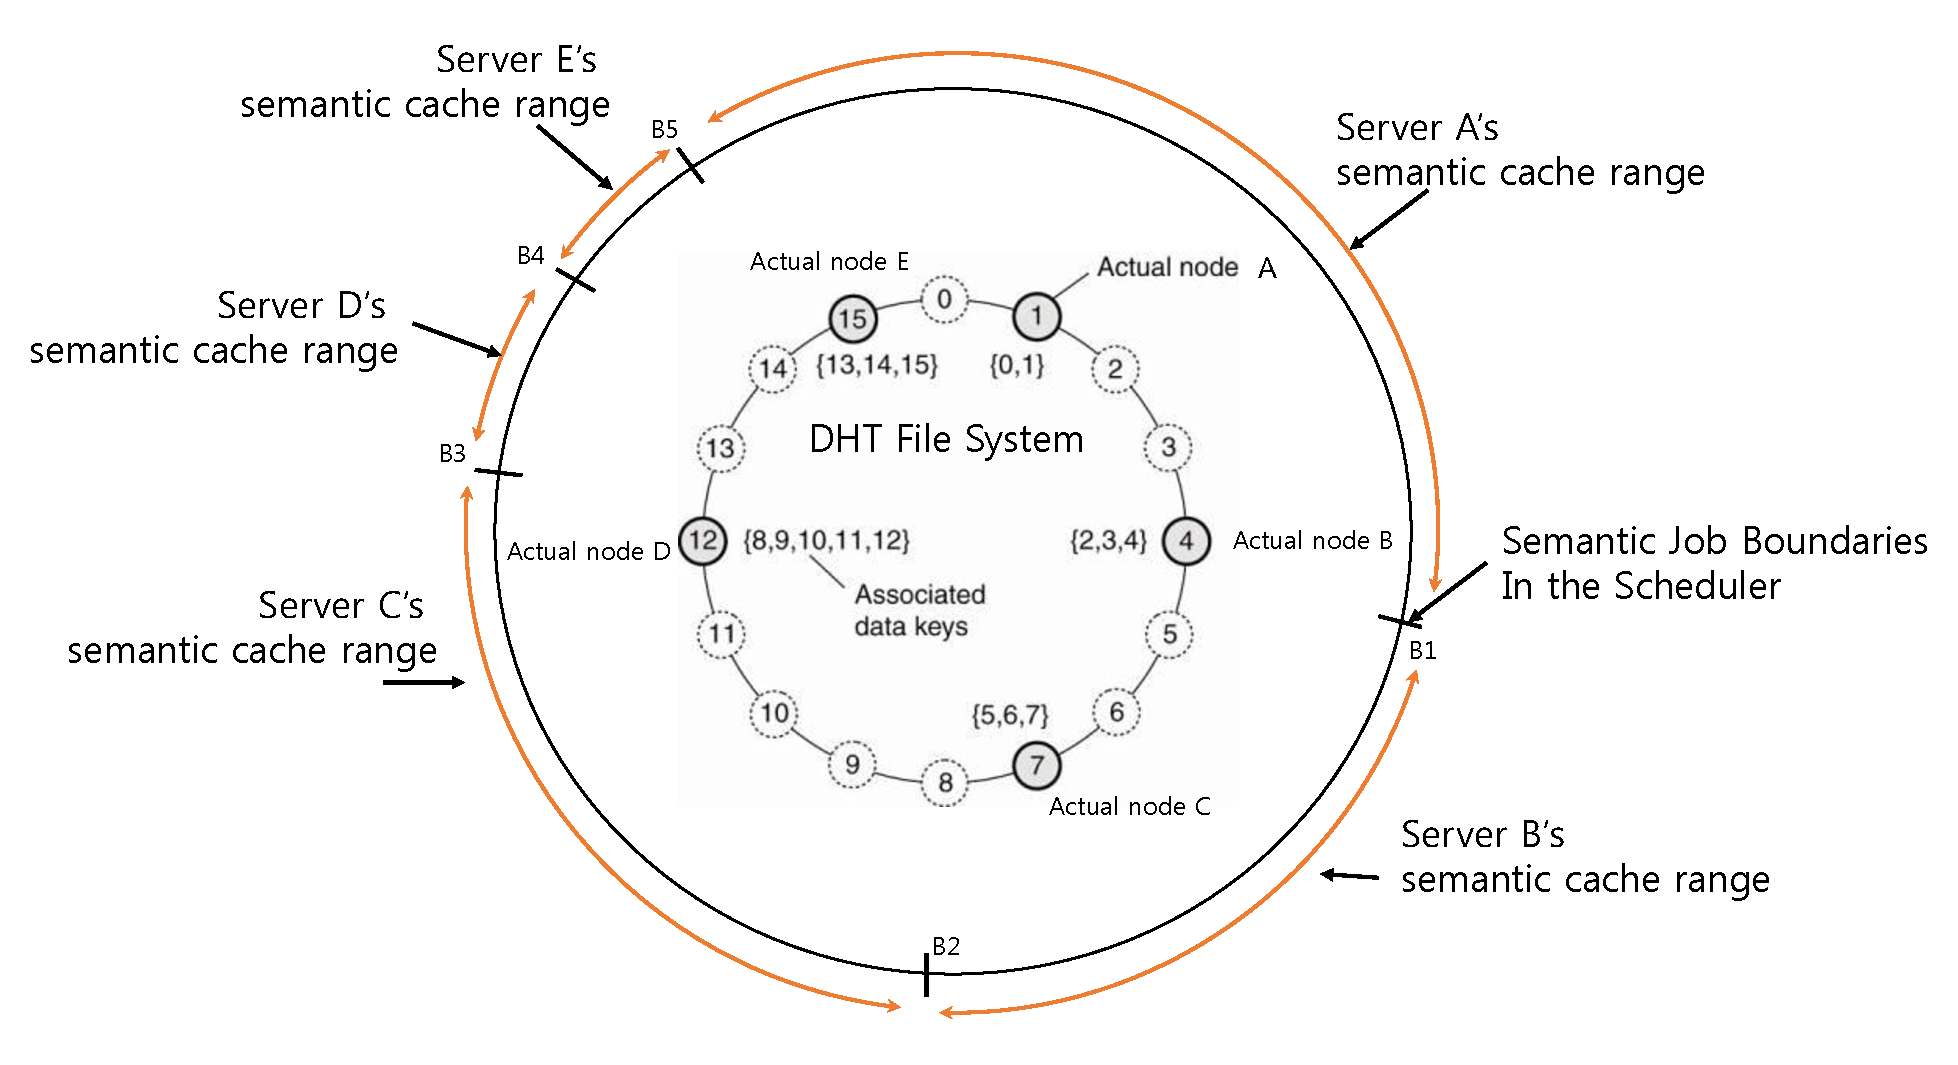
\includegraphics[width=.48\textwidth]{arch.eps}
\caption{\textit{Two layers structure of back-end servers.}}
\label{fig:fig1}
\end{figure}

%Previous policies
%Starting on the basis that in a tipical use of a DQP, the probability of an 
%access near located data that the previous access. 

%Our middle-ware makes some assumsions. Firstly considering an hard-disk
%as a bottle-neck and providing a much faster network.


We propose a framework composed of a set of accesible front-end servers 
and a collection of back-end caching servers organized in a two layers peer-to-peer structure.
%UniDQP can be seen as a two layers hybrid peer-to-peer system with scheduler.


%one outer layer which reflects the cached dataset,
%and one inner layer which represent the full dataset dispersed among the existing
%hard-disks.

%the where while the every 
%back-end server has a fixed section of the data store in its hard-disk, every data cached
%in the system is accessible from every back-end node.
%The most important property of this layer is that

\subsubsection{Inner layer}
It consists in a set of not mutable static segments which represents the range of the dataset corresponding
to each back-end server. This layer is visible from every back-end servers through its hashing lookup table.

\subsubsection{Outer layer}
Analogously, we propose a non-static layer divided in mutable boundaries which 
represents the current status of the cached data. This layer is not completely visible, where
in contrast to the inner layer, each back-end node only knows its boundary and neighbors.
Those boundaries are in a continuous movement due to our spacial algorithm.

%is not static and its continuously changing, also a back-end
%server only knows about its own boundaries.

%\subsection{Hashing lookup table}
%In order to locate the correct back-end server. We propose an share and distributed 
%lookup table which store for each data the server where it belongs.
%
%\subsection{Pop policy}
%One of the most important functionability in systems with large dataset is the
%discarding policy, since a backend node only can cache a small percentage of its dataset.
%UniDQP will simply discard those nodes whichthe least-recently-used or less likely to be accessed
%data to its closer neighbor backend server.
%has an lookup table which 

\subsection{Data migration}
An intensive use of data migration is necessary to guarantee a high cohesion between the 
front-end and back-end servers. Our framework accomplish two main problems making use of this policy:

\subsubsection{Overlap of the boundaries}
Due to a continous movement of the boundaries of the outer layer, at some point the data located near by
its boundary could be out of its original range, for this reason our framework corrects the overlap migrating
overlapped data to the range where it belongs.

\subsubsection{Requesting data}
As the ranges are continously moving, the scheduler can not know accurately which back-end node contains
the requested data. In order to overcome this problems our framework provide a hashing lookup table
to each back-end server indicating which range in the inner layer contains the requested data. 
In case of failure of the scheduler, the requested data will be readed from the corresponing back-end server
and cached in the back-end server selected by the scheduler.

%where whenever a query arrives in a given back-end server,
%in case that such back-end server does not contain that data, it consults its lookup table and redirects
%the query to the back-end node whose has assign the range of dataset in the inner layer which contains
%that query. Also, this migration process is use to balance the system.


%On the other hand, our framework needs a scheduler to redirect the queries and compute the boundaries.

\begin{figure}
\centering 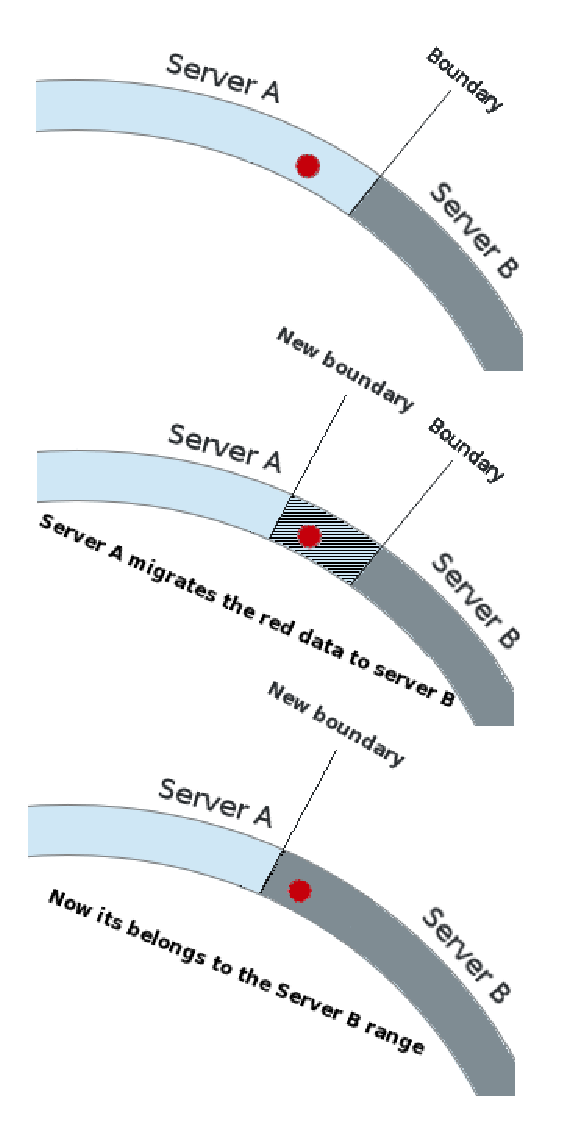
\includegraphics[width=.20\textwidth]{graphic1.eps}
\caption{\textit{Two layers structure of back-end servers.}}
\label{fig:fig2}
\end{figure}

%Our middle-ware performance is based on the data migration between the back-end servers.
%In several cases it will migrate data. Firstly, whenever the cache is full it will migrate
%at first the farthest element from the EMA point in the cache the least-recently-accessed data


%actual policy

%\begin{figure*}[!ht]
%\centering
%\subfigure[Query Response Time]{
%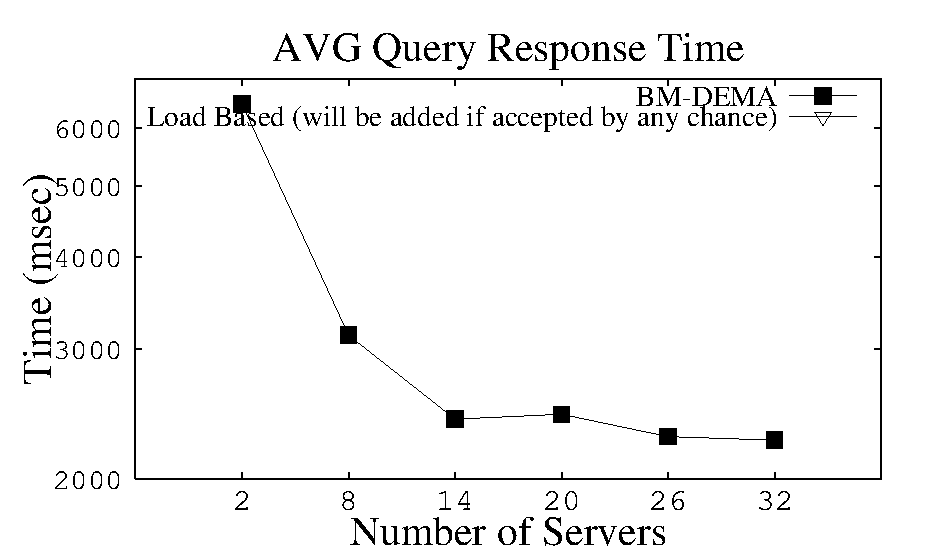
\includegraphics[width=.38\textwidth]{nservers.qwet.eps}
%\label{fig:real-qwet}
%}
%\subfigure[Hit Ratio]{
%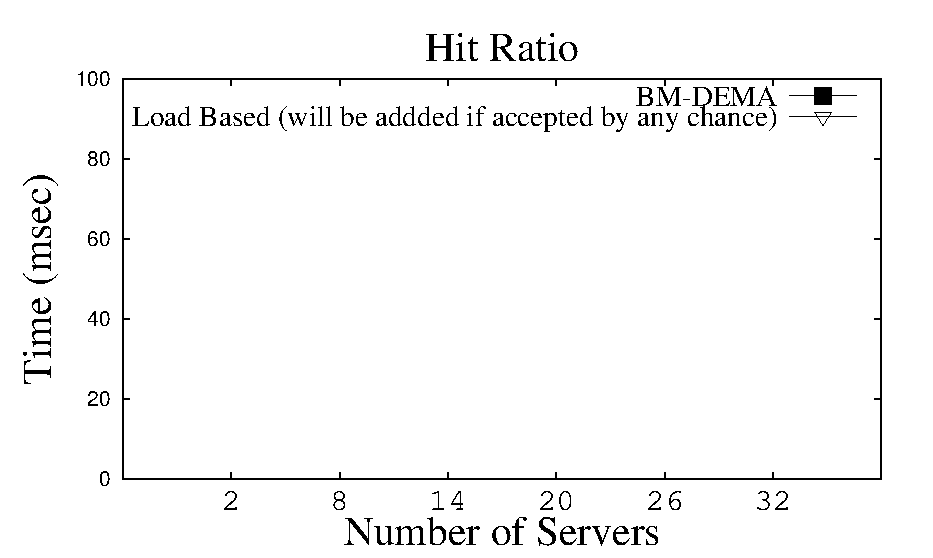
\includegraphics[width=.38\textwidth]{nservers.hit.eps}
%\label{fig:real-balance}
%}
%\caption{\textit{Query Response Time and Hit Ratio with Varying \# of Back-end Servers}}
%\label{fig:nservers}
%\end{figure*}


